%%%%%%%%%%%%%%%%%%%%%%%%%%%%%%%%%%%%%%%%%
% Lachaise Assignment
% LaTeX Template
% Version 1.0 (26/6/2018)
%
% This template originates from:
% http://www.LaTeXTemplates.com
%
% Authors:
% Marion Lachaise & François Févotte
% Vel (vel@LaTeXTemplates.com)
%
% License:
% CC BY-NC-SA 3.0 (http://creativecommons.org/licenses/by-nc-sa/3.0/)
% 
%%%%%%%%%%%%%%%%%%%%%%%%%%%%%%%%%%%%%%%%%

%----------------------------------------------------------------------------------------
%	PACKAGES AND OTHER DOCUMENT CONFIGURATIONS
%----------------------------------------------------------------------------------------

\documentclass{article}

%%%%%%%%%%%%%%%%%%%%%%%%%%%%%%%%%%%%%%%%%
% Lachaise Assignment
% Structure Specification File
% Version 1.0 (26/6/2018)
%
% This template originates from:
% http://www.LaTeXTemplates.com
%
% Authors:
% Marion Lachaise & François Févotte
% Vel (vel@LaTeXTemplates.com)
%
% License:
% CC BY-NC-SA 3.0 (http://creativecommons.org/licenses/by-nc-sa/3.0/)
% 
%%%%%%%%%%%%%%%%%%%%%%%%%%%%%%%%%%%%%%%%%

%----------------------------------------------------------------------------------------
%	PACKAGES AND OTHER DOCUMENT CONFIGURATIONS
%----------------------------------------------------------------------------------------

\usepackage{amsmath,amsfonts,stmaryrd,amssymb} % Math packages

\usepackage{enumerate} % Custom item numbers for enumerations
\usepackage{enumitem}
\usepackage[ruled]{algorithm2e} % Algorithms

\usepackage[framemethod=tikz]{mdframed} % Allows defining custom boxed/framed environments

\usepackage{listings} % File listings, with syntax highlighting
\lstset{
	basicstyle=\ttfamily, % Typeset listings in monospace font
}

%----------------------------------------------------------------------------------------
%	DOCUMENT MARGINS
%----------------------------------------------------------------------------------------

\usepackage{geometry} % Required for adjusting page dimensions and margins

\geometry{
	paper=a4paper, % Paper size, change to letterpaper for US letter size
	top=2.5cm, % Top margin
	bottom=3cm, % Bottom margin
	left=2.5cm, % Left margin
	right=2.5cm, % Right margin
	headheight=14pt, % Header height
	footskip=1.5cm, % Space from the bottom margin to the baseline of the footer
	headsep=1.2cm, % Space from the top margin to the baseline of the header
	%showframe, % Uncomment to show how the type block is set on the page
}

%----------------------------------------------------------------------------------------
%	FONTS
%----------------------------------------------------------------------------------------

\usepackage[utf8]{inputenc} % Required for inputting international characters
\usepackage[T1]{fontenc} % Output font encoding for international characters

\usepackage{XCharter} % Use the XCharter fonts

%----------------------------------------------------------------------------------------
%	COMMAND LINE ENVIRONMENT
%----------------------------------------------------------------------------------------

% Usage:
% \begin{commandline}
%	\begin{verbatim}
%		$ ls
%		
%		Applications	Desktop	...
%	\end{verbatim}
% \end{commandline}

\mdfdefinestyle{commandline}{
	leftmargin=10pt,
	rightmargin=10pt,
	innerleftmargin=15pt,
	middlelinecolor=black!50!white,
	middlelinewidth=2pt,
	frametitlerule=false,
	backgroundcolor=black!5!white,
	frametitle={Command Line},
	frametitlefont={\normalfont\sffamily\color{white}\hspace{-1em}},
	frametitlebackgroundcolor=black!50!white,
	nobreak,
}

% Define a custom environment for command-line snapshots
\newenvironment{commandline}{
	\medskip
	\begin{mdframed}[style=commandline]
}{
	\end{mdframed}
	\medskip
}

%----------------------------------------------------------------------------------------
%	FILE CONTENTS ENVIRONMENT
%----------------------------------------------------------------------------------------

% Usage:
% \begin{file}[optional filename, defaults to "File"]
%	File contents, for example, with a listings environment
% \end{file}

\mdfdefinestyle{file}{
	innertopmargin=1.6\baselineskip,
	innerbottommargin=0.8\baselineskip,
	topline=false, bottomline=false,
	leftline=false, rightline=false,
	leftmargin=2cm,
	rightmargin=2cm,
	singleextra={%
		\draw[fill=black!10!white](P)++(0,-1.2em)rectangle(P-|O);
		\node[anchor=north west]
		at(P-|O){\ttfamily\mdfilename};
		%
		\def\l{3em}
		\draw(O-|P)++(-\l,0)--++(\l,\l)--(P)--(P-|O)--(O)--cycle;
		\draw(O-|P)++(-\l,0)--++(0,\l)--++(\l,0);
	},
	nobreak,
}

% Define a custom environment for file contents
\newenvironment{file}[1][File]{ % Set the default filename to "File"
	\medskip
	\newcommand{\mdfilename}{#1}
	\begin{mdframed}[style=file]
}{
	\end{mdframed}
	\medskip
}

%----------------------------------------------------------------------------------------
%	NUMBERED QUESTIONS ENVIRONMENT
%----------------------------------------------------------------------------------------

% Usage:
% \begin{question}[optional title]
%	Question contents
% \end{question}

\mdfdefinestyle{question}{
	innertopmargin=1.2\baselineskip,
	innerbottommargin=0.8\baselineskip,
	roundcorner=5pt,
	nobreak,
	singleextra={%
		\draw(P-|O)node[xshift=1em,anchor=west,fill=white,draw,rounded corners=5pt]{%
		Question \theQuestion\questionTitle};
	},
}

\newcounter{Question} % Stores the current question number that gets iterated with each new question

% Define a custom environment for numbered questions
\newenvironment{question}[1][\unskip]{
	\bigskip
	\stepcounter{Question}
	\newcommand{\questionTitle}{~#1}
	\begin{mdframed}[style=question]
}{
	\end{mdframed}
	\medskip
}

%----------------------------------------------------------------------------------------
%	WARNING TEXT ENVIRONMENT
%----------------------------------------------------------------------------------------

% Usage:
% \begin{warn}[optional title, defaults to "Warning:"]
%	Contents
% \end{warn}

\mdfdefinestyle{warning}{
	topline=false, bottomline=false,
	leftline=false, rightline=false,
	nobreak,
	singleextra={%
		\draw(P-|O)++(-0.5em,0)node(tmp1){};
		\draw(P-|O)++(0.5em,0)node(tmp2){};
		\fill[black,rotate around={45:(P-|O)}](tmp1)rectangle(tmp2);
		\node at(P-|O){\color{white}\scriptsize\bf !};
		\draw[very thick](P-|O)++(0,-1em)--(O);%--(O-|P);
	}
}

% Define a custom environment for warning text
\newenvironment{warn}[1][Warning:]{ % Set the default warning to "Warning:"
	\medskip
	\begin{mdframed}[style=warning]
		\noindent{\textbf{#1}}
}{
	\end{mdframed}
}

%----------------------------------------------------------------------------------------
%	INFORMATION ENVIRONMENT
%----------------------------------------------------------------------------------------

% Usage:
% \begin{info}[optional title, defaults to "Info:"]
% 	contents
% 	\end{info}

\mdfdefinestyle{info}{%
	topline=false, bottomline=false,
	leftline=false, rightline=false,
	nobreak,
	singleextra={%
		\fill[black](P-|O)circle[radius=0.4em];
		\node at(P-|O){\color{white}\scriptsize\bf i};
		\draw[very thick](P-|O)++(0,-0.8em)--(O);%--(O-|P);
	}
}

% Define a custom environment for information
\newenvironment{info}[1][Info:]{ % Set the default title to "Info:"
	\medskip
	\begin{mdframed}[style=info]
		\noindent{\textbf{#1}}
}{
	\end{mdframed}
}
 
\usepackage{hyperref}
\hypersetup{colorlinks=true, citecolor={blue}}
\usepackage{natbib}
\usepackage{comment}
\usepackage{float}

\newcommand{\msun}{\ensuremath{M_\odot}}
\newcommand{\rsun}{\ensuremath{R_\odot}}
\newcommand{\be}{\begin{equation}}
\newcommand{\ee}{\end{equation}}
\newcommand{\tder}[2]{\frac{{\rm d}#1}{{\rm d}#2}}

% Include the file specifying the document structure and custom commands
\usepackage{enumitem}
%----------------------------------------------------------------------------------------
%	ASSIGNMENT INFORMATION
%----------------------------------------------------------------------------------------

\title{Stellar Structure and Evolution: MESA Project} 
\author{Mahdi N. Ziyazi, Adam Parkosidis, Gabriel Simion}
\date{University of Amsterdam 2021} 

%----------------------------------------------------------------------------------------

\begin{document}

\maketitle 


\section*{Introduction}

In this project, we are interested in studying various types of stars during different evolution phases. We evaluate the changes of core abundances, evolution in the central temperature-density plane and in the Hertzsprung-Russel diagram. In addition, we discuss the evolution of two stars in the Kippenhahn diagram. In order to do these tasks, we have performed a variety of simulations using the Modules for Experiments in Stellar Astrophysics (MESA) code, developed by \citet{paxton2010modules}. The plots presented in this report were made using the Matplotlib module from Python.



\section{Time evolution of the central abundances for a massive star}

\begin{comment}

\begin{figure}
    \centering
    \includegraphics[width=10cm]{plots/H_HE.pdf}
    \caption{Central abundances of H and He as a function of time of a star of 15\msun}
    \label{fig:abundances1}
\end{figure}
\begin{figure}
    \centering
    \includegraphics[width=10cm]{plots/N_O_C.pdf}
    \caption{Central abundances of C, N \& O as a function of time of a star of 15\msun}
    \label{fig:abundances2}
\end{figure}
\begin{figure}
    \centering
    \includegraphics[width=10cm]{plots/He_C_O.pdf}
    \caption{Central abundances of C, N \& O as a function of time of a star of 15\msun, zooming in on the central helium burning phase.}
    \label{fig:abundances3}
\end{figure}

\end{comment}

\begin{enumerate}

    \begin{figure}[H]
    \centering
    \includegraphics[width=10cm]{plots/H_HE.pdf}
    \caption{Central abundances of H and He as a function of time of a star of 15\msun}
    \label{fig:abundances1}
    \end{figure}

    \item Fig \ref{fig:abundances1}, shows the evolution of the mass fraction of the central hydrogen and helium for 15$M_{\odot}$ star until the end of the main-sequence. In the beginning, the mass fraction of hydrogen and helium is roughly 0.70 and 0.28 respectively. As the star grows older, it burns hydrogen in the core and produces helium through the CNO-cycle:
    $$
\begin{aligned}
&{ }^{12} \mathrm{C}+{ }^{1} \underline{\mathrm{H}} \rightarrow{ }^{13} \mathrm{~N}+\gamma\\
&{ }^{13} \mathrm{~N} \rightarrow{ }^{13} \mathrm{C}+\mathrm{e}^{+}+v\\
&{ }^{13} \mathrm{C}+{ }^{1} \underline{\mathrm{H}} \rightarrow{ }^{14} \mathrm{~N}+\gamma\\
&{ }^{14} \mathrm{~N}+{ }^{1} \underline{\mathrm{H}} \rightarrow{ }^{15} \mathrm{O}+\gamma\\
&{ }^{15} \mathrm{O} \rightarrow{ }^{15} \mathrm{~N}+\mathrm{e}^{+}+v\\
&{ }^{15} \mathrm{~N}+{ }^{1} \underline{\mathrm{H}} \rightarrow{ }^{12} \mathrm{C}+{ }^{4} \underline{\underline{\mathrm{He}}}\\
&\ \ \ \ \ \ \ \ \ \ \ \ \ \ \ \rightarrow{ }^{16} \mathrm{O}+\gamma\\ \\
&{ }^{16} \mathrm{O}+{ }^{1} \underline{\mathrm{H}} \rightarrow{ }^{17} \mathrm{~F}+\gamma\\ 
&{ }^{17} \mathrm{~F} \rightarrow{ }^{17}
\mathrm{O}+\mathrm{e}^{+}+v\\
&{ }^{17} \mathrm{O}+{ }^{1} \underline{\mathrm{H}} \rightarrow{ }^{14} \mathrm{~N}+{ }^{4} \underline{\underline{\mathrm{He}}}
\end{aligned}
$$
    
    Therefore, gradually the mass fraction of helium increases while the mass fraction of hydrogen decreases. The dashed line marks the end of the main-sequence where the hydrogen mass fraction in the core reaches a negligible value($X = 0.01$) while the the amount of helium reaches its maximum.  
    
    \begin{figure}[H]
    \centering
    \includegraphics[width=10cm]{plots/N_O_C.pdf}
    \caption{Central abundances of C, N \& O as a function of time of a star of 15\msun}
    \label{fig:abundances2}
    \end{figure}
    
    \item In Fig \ref{fig:abundances2}, we can see how the mass fractions of carbon, nitrogen, and oxygen varies while the star is in the main-sequence phase. Carbon seems to have remained constant during this phase which also can be seen in the CNO-cycle. Carbon is consumed during the cycle in the reaction ${ }^{12} \mathrm{C}(p, \gamma)^{13} \mathrm{N}$  but later it is produced again through reaction ${ }^{15} \mathrm{N}(p,\alpha) ^{12} \mathrm{C}$. Therefore, its mass fraction remains almost constant. \\
    \\
    In the beginning, Nitrogen ($^{14}$N) is produced through the reaction ${ }^{13} \mathrm{C}(p, \gamma)^{14} \mathrm{N}$ but later it is consumed in the CN-part of the cycle through ${ }^{14} \mathrm{N}(p, \gamma)^{15} \mathrm{O}$.  This latter reaction is the bottleneck of the CNO-cycle and it takes place very slowly. This implies that the rate of Nitrogen consumption is slower than its production, allow for Nitrogen to pile up.
    Moreover, Nitrogen is also produced in the second part of the CNO-cycle through the reaction ${ }^{17} \mathrm{O}(p, \alpha)^{14} \mathrm{N}$ which also increase the mass fraction of Nitrogen through this phase. 
    \\
    \\
    The red curve represents the trend of oxygen mass fraction. As we can see, its mass fraction is decreasing from the beginning, and this agrees with our theory. There is only one occasion in CNO-cycle that oxygen could be produced and that is through reaction  ${ }^{15} \mathrm{N}(p, \gamma)^{16} \mathrm{O}$. However, the chance of this reaction to occur is very low. Therefore, the population of the oxygen would decrease through the reaction ${ }^{16} \mathrm{O}(p, \gamma)^{17} \mathrm{F}$ in the second part of the CNO-cycle as seen in Fig \ref{fig:abundances2}.
    
    \begin{figure}[H]
    \centering
    \includegraphics[width=10cm]{plots/He_C_O.pdf}
    \caption{Central abundances of C, N \& O as a function of time of a star of 15\msun, zooming in on the central helium burning phase.}
    \label{fig:abundances3}
    \end{figure}
    
    \item In Fig \ref{fig:abundances3}, our focus is on the evolution of the helium burning phase of the star. The helium in the core of this stars goes through what is known as {\it triple-$\alpha$} reaction: 
    \\
    \\
    $3^{4} \mathrm{He} \rightarrow{ }^{12} \mathrm{C}+\gamma$. \\
    \\
    As seen in this Fig, the population of helium is decreasing while at the same time,  the population of carbon is increasing which agrees with the {\it triple-$\alpha$} reaction. However, once the carbon becomes more abundant, it reacts with helium to produce oxygen:
    \\
    \\
    ${ }^{12} \mathrm{C}+{ }^{4} \mathrm{He} \rightarrow{ }^{16} \mathrm{O}+\gamma$
    \\
    \\
    We believe that this latter reaction becomes more effective at around $t \approx 11.65 \ [Myrs]$, so we have a slight change in the slopes of the plots at that specific point. After this point, there would be a competition between the two reactions to consume helium. Since the reaction ${ }^{12} \mathrm{C}(\alpha, \gamma)^{16} \mathrm{O}$ only needs one helium, it is more probable to occur, and wins the competition. So the production of carbon slows down while its consumption rises, and as a result more oxygen is produced. This process will carry on until the carbon production through {\it triple-$\alpha$} reaction stops (local maximum on the graph). This happens because the mass fraction of helium has reached a low point that it is not possible anymore for the {\it triple-$\alpha$} reaction to take place. Therefore, only ${ }^{12} \mathrm{C}(\alpha, \gamma)^{16} \mathrm{O}$ would take place and consume the remaining helium to produce oxygen. By the end of the helium burning, oxygen is the most dominant element in the core, followed by carbon. 
\end{enumerate}


\section{A Hertzsprung-Russell diagram from 1 to 12~\msun}


\begin{enumerate}
    \item There are different parameters which can be used to exclude the pre-main-sequence. Yet, we chose to use the criterion based on the thermal equilibrium. Once the hydrogen nuclear fusion from the core sets in, it produces energy at the same rate as the one to which energy is radiated at the surface ($L_{nuc} \geq 0.99L$). Thus, the thermal equilibrium is reached. From this point on, the gravitational contraction halts and the star enters in the main-sequence phase. 
    
    \begin{figure}[H]
    \centering
    \includegraphics[width=10cm]{plots/HR_lowZ.pdf}
    \caption{HR diagram for five stars of different mass and for a 7 \msun star with $0.02 \; Z_{\odot}$}
    \label{fig:HR1}
    \end{figure}
    
    \item In Fig \ref{fig:HR1} we see the evolution tracks during the main-sequence phase for five stars with different masses. We also bring into discussion the evolution of a star with a lower metallicity. The main-sequence evolution begins at ZAMS (marked with black dots), when the thermal equilibrium is reached. During this phase, the hydrogen is fused into $^4$He. Independently on the ongoing reaction channel (pp or CNO), the luminosity of the star will increase during the MS phase (L$\,\propto\,\mu^{4}\,M^3$). This is due to the change in the core's composition, as the H is fused into He ($\mu$ increases). However, the way in which the star evolves through the MS-phase depends on its mass. 
    
    Stars with masses M\,$\geq$\,1.3\,M$_\odot$ are driven by the CNO-cycle ($\epsilon_{CNO}\,\propto\,\rho\,T^{18}$). As the luminosity increases over time, the energy produced in the core needs to increase too, in order to maintain the TE. However, due to the high dependence on the central temperature of $\epsilon_{CNO}$, a small change of T$_c$ will have a tremendous effect on the energy production rate, which would take out the star from HE and TE. Thus, T$_c$ needs to remain almost constant in time. The way in which such a star keeps T$_c$ constant, while $\mu$ increases, is to decrease the pressure inside the core by expanding the envelope on the nuclear time-scale. Hence, these stars evolve through larger radii and lower T$_{eff}$.
    
    Also, the stars driven by the CNO-cycle have convective cores, since the energy produced is too large to be transported by radiation ($\nabla_{rad} > \nabla_{ad}$). One effect of the convection on the evolution is that the MS-lifetime is extended (H is brought from the envelope inside the core). Another effect is that as the core approaches the end of H-burning, the reactions suddenly cease in the whole core. The star responds to this sudden stop of energy production by a more violet contraction, giving rise to the observed "hook" feature. 
    
    If the star has a mass lower that $\sim 1.3 M_\odot$, the hydrogen is mainly fused in the proton-proton chain. This is the case of the 1 M$_\odot$ star, which has a different track compared to the other stars. The reason why is this happening is because the energy production rate of the pp-chain is less sensitive to the temperature ($\epsilon_{pp}\,\propto\,\rho\,T^{4}$). Consequently, the increasing of the energy production rate (as the luminosity increases over time) can be done by rising T$_c$, since this would have a lower effect on $\epsilon_{pp}$. Moreover, if the TE and HE can be maintained by changing T$_c$, the envelope doesn't have to expand and the star will evolve with an almost constant radius.
    
    The energy produced in the pp-chain is lower than for the CNO-cycle. Hence, the core of these stars is completely radiative (excepting those fully convective low-mass stars). Since the material is not mixed during this phase, the H fraction inside the core will have a gradient. Thus, as the end of H-burning approaches, the reactions will be ceased gradually (from the centre to the edge of the core). This means that the contraction will also occur smoothly and the "hook" feature is not observed.
    
    \item  The Hertzsprung-Russel diagram is a logarithmic representation of the surface luminosity (or absolute magnitude) of a star as a function of its effective temperature (or spectral type). It is used to study the evolution of a star during different phases (from the pre-main sequence up to the late phases). It is divided into five different regions, namely the main-sequence, the red-giant branch, the horizontal-giant branch, the asymptotic-giant branch and the region of degenerate stars (WD). Depending on its mass, a star will evolve through some of these regions during its life as a result of the interplay between the nuclear reactions and the gravitational contraction. 
    
    In Fig \ref{fig:HR1} we have also plotted the evolution track of a 7\,M$_{\odot}$ star with a 1\% solar metallicity. One can see a shift towards higher temperature, but at constant luminosity. Due to its high mass (7\,M$_{\odot}$), the hydrogen-core burning is driven by the CNO-cycle. However, the effect of a lower metallicity is that the reaction rate is lower, which means that at the same temperature, the produced energy is smaller. However, both stars of 7\,M$_\odot$ have the same luminosity (L\,$\propto $\,M$^3$). Thus, in order to have the same amount of energy produced in the core, the star with a lower Z needs to contract, so that the core temperature (and consequently the reactions rate) increases. This contraction means that the radius will become smaller, as it can be seen in the plot. 
    
    \begin{figure}[H]
    \centering
    \includegraphics[width=10cm]{plots/HR_5M.pdf}
    \caption{HR diagram of a 5 \msun star with annotations of the different evolutionary phases}
    \label{fig:HR2}
    \end{figure}
    
    
    \item Fig \ref{fig:HR2} indicates the evolution of a 5$\msun$ star from the beginning of the main-sequence until the end of the helium burning phase. The evolution has been further categorized in to four sections: main-sequence (green), Hertzsprung gap (orange), red giant branch (red) and blue loop (blue). The answers 5 and 6 give also a a detailed explanation of the evolution through out these four sections.

    
    \item  (a) The two phases of the star's contraction apart from the pre-main sequence are: the second part of the main-sequence where we observe the ``hook'' feature and the evolution after the ignition of helium at point {\it E} until the point {\it F}. This second phase includes the second part of the red giant branch and the first part of the blue loop. 
    
    (b) The reasoning behind the first contraction is this:  A 5$\msun$ star has a convective core and this leads to a constant feeding of the core with hydrogen from the upper layers. Thus, the fraction of hydrogen keeps reducing through the CNO-cycle in the whole core. This process takes place suddenly from the center towards the limb of the core. Consequently, the energy generation rate would normally decrease due to the sudden depletion of hydrogen in the core, which also diminishes the thermostatic action of the CNO reactions, threatening the thermal equilibrium of the star. In response the temperature of the core ($T_c$) needs to increase in order to keep the same energy generation rate. The ideal gas law implies that $\frac{P_c}{\rho_c} \propto \frac{T_c}{\mu}$, thus the pressure exerted on the core by the envelope must increase leading to the contraction of the star which also leads to higher effective temperature ($T_{eff}$). This is evident in the second part of the main-sequence in Fig. \ref{fig:HR2}, where we observe the ``hook'' feature. 
    
    The reasoning behind the second contraction is this: At point {\it E} the helium core has reached temperatures $T_c \sim 10^8 K$ where the helium ignites, and  the system reaches thermal equilibrium again. The fusion of helium in the core stops the core's contraction and starts to change its composition. Helium starts to convert to carbon via the {\it triple-$\alpha$} process and as the abundance of carbon builds up it starts to react with the helium itself producing oxygen,  Fig. \ref{fig:abundances3}. The convective envelope now starts to contract. At the beginning this contraction happens under nearly constant effective temperature. To fully explain this behavior we need to dive in more details. The {\it triple-$\alpha$} reaction is extremely sensitive to the temperature $\epsilon_{nuc,3\alpha} \propto \rho^2 T^{40}$. Once again, this means that a change in $T_c$ will result to a big change in the generation rate and consequently violate the thermal equilibrium. As helium is converted into heavier elements, the mean molecular weight $\mu$ in the core increases, thus the generated power by the core, $L \propto \mu^4 M_c^{3}$ increases too (on $\tau_{nuc}$). Following the same reasoning as during the main sequence, for an ideal gas $\frac{P_c}{\rho_c} \propto \frac{T_c}{\mu}$, the layers surrounding the core must expand to keep $T_c \sim const.$ . The important difference here is that there is a shell in which hydrogen burning takes places via the CNO-cycle. Consequently, the expansion of the layers around the core will result to the increase of the pressure that is exerted by the latter towards that shell. The thermostatic behavior of the CNO-cycle once again tries to maintain the thermal equilibrium, $T_{sh} \sim const.$ in the shell, and because $\frac{P_{sh}}{\rho_{sh}} \propto \frac{T_{sh}}{\mu_{sh}}$ the pressure by the envelope towards the hydrogen burning shell must increase. This leads to the envelope's contraction and consequently to the reduction of the luminosity $L$ as can be seen in Fig. \ref{fig:HR2}, which is still determined by the conditions in the photosphere because of the convective envelope. The contraction takes place until point {\it F}, but it is evident that the rate of the contraction becomes lower as the star moves towards {\it F}. In reality the temperature in the envelope slowly rises as the star reaches the end of the red-giant branch (transition from the red line to the blue line), thus the opacity also rises and the envelope becomes gradually less convective and more radiative. This is happening because not all the layers from the hydrogen burning shell and above are convective, but there is a small part at the bottom of the envelope that is still radiative. Hence, the helium burning acts now as a second source of energy inside the star. As the latter moves towards the transition point is already in thermal equilibrium and the virial theorem indicates that as the envelope contracts must rise its internal energy, thus rise its temperature. Consequently, the radiative layers above the core (not the hydrogen burning shell) are gradually heated erasing the convection from inside towards the surface of the star. From the transition point on the star enters the blue loop with a radiative envelope, which keeps contracting but the contraction is slowly decelerating, and a gradually increasing effective temperature. Hence, the luminosity starts to rise, because has a stronger dependence on the effective temperature than on the radius ($L \propto R^2 T_{eff}^4$). This is evident in Fig. \ref{fig:HR2}.
    
    \item (a) Evolution across the Hertzsprung gap: Letters {\it B} and {\it C} indicate the end of the main-sequence, where the hydrogen in the core has been depleted, and the beginning of the hydrogen burning in a shell around the core respectively. From that point on, the star enters the Hertzsprung gap branch. Considering convective overshooting, for a 5$\msun$ star the mass of the hydrogen depleted core is $\geq$ S-C limit, so the core contracts in $\tau_{KH}$ in an attempt to reach thermal equilibrium. The virial theorem indicates that half of the gravitational energy ($E_{grav}$) is converted to internal energy ($E_{int}$) raising the central temperature ($T_c$), while the other half is escaping as luminosity ($L$) from the core. Furthermore, the hydrogen burning in the shell around the core also produces energy via the CNO-cycle. A significant fraction of the energy from these two sources acts as the work applied towards the envelope leading to the expansion of the latter under hydrostatic equilibrium, while the expansion itself results to the temperature in the envelope being reduced. Simultaneously, the abundance of hydrogen in the shell is reducing making the shell gradually thinner, while the produced helium is adding gradually mass to the helium core speeding up its contraction. The aforementioned behavior is evident in Fig. \ref{fig:HR2} as the star moves towards bigger radius ($R$) and lower effective temperature ($T_{eff}$). The total luminosity ($L$) overall reduces. First, because a significant fraction of the produced energy is being absorbed by the expanding envelope and second luminosity has a stronger dependence on the effective temperature than on the radius ($L \propto R^2 T_{eff}^4$). An important thing to mention is that during this phase the temperature in the core ($T_c$) is raising up and should not be confused with the behavior of the ($T_{eff}$). As the star moves towards {\it D} the reduction of the effective temperature ($T_{eff}$) results to the raise of the opacity ($\kappa$) in the envelope, thus the energy transport through radiation becomes less efficient ($\nabla_{rad} \propto \kappa$), while gradually the envelope becomes convective.
    
    (b) Ascend of the (first) giant branch: Letter {\it D} marks the beginning of the red giant branch. At this point, the star enters this phase with high opacity in the envelope, a continuously contracting core and a convective envelope which continuously expands. To explain this seemingly contradicting behavior ($L \nearrow$ while $\kappa \nearrow \; \&  \; T_{eff} \searrow$) we need to consider the impact of convection in the expansion rate of the envelope. First, having a convective envelope means that the luminosity is determined by the conditions in a thin radiative layer at the edge of the star, the photosphere, where photons can escape (mostly determined by the opacity, which is a function of the density, $\rho_R$, and temperature $T_{eff},$ in this layer).  As we already discussed the expansion and consequently the changes in the effective temperature ($T_{eff}$) take place on a thermal timescale $\tau_{KH}$, because it is a result of the contraction of the core (``mirror principle''), but the bulk motion of the gas (convection) in the envelope occurs in a timescale $\tau_{conv}$, where $\tau_{conv} << \tau_{KH}$. This means that even though convection can efficiently transfer a large amount of energy, this occurs in nearly constant effective temperature $T_{eff}$, the process is adiabatic. Fig. \ref{fig:HR2} indicates that the luminosity is increasing considerably during this phase of the evolution and for this to happen under nearly constant effective temperature, the increase of the radius ($R$) must accelerate ($L \propto R^2 T_{eff}^4$). This is exactly what we see in Fig. \ref{fig:HR2}, with the radius at {\it D} being $\sim 25 R_{\odot}$ and at {\it E} being $\sim 60 R_{\odot}$, while $T_{eff} \sim 3.7$ and $T_{eff} \sim 3.63$ respectively; To further evaluate the impact of the convective envelope on the expansion rate, we can also compare the expansion from {\it C-D} with the one from {\it D-E}, both occur in thermal timescale $\tau_{KH}$.

    A more intuitive explanation for the rapid expansion under nearly constant effective temperature is this: As a parcel of hot gas comes from deeper layers towards layers with lower density, it needs to expand and push the surrounding gas out of the way. In order to do that, it requires energy. The only form of energy available to the gas is its own heat. Hence, when the parcel of gas expands, its pressure drops, and it uses its own heat energy to push away surrounding gas and make room for its own expansion, therefore its temperature drops. The gas does not exchange heat with its environment by any mechanism during this process, even though the gas cools. The overall result, is that the pressure of the convective gas is a function only of density (thus polytropic EOS) and independent of the temperature. The heat energy of the parcel of gas is given to the pressure which pushes the surrounding gas and that is the reason behind fast expansion of the envelope after point {\it D}, which results to the steep increase of the luminosity. The second part of the red-giant branch has already being described above (5b).
    

    (c) blue loop: From the transition point on (where the red line becomes blue)  the star enters the blue loop with a radiative envelope, which keeps contracting but the contraction is slowly decelerating, and gradually increasing the effective temperature. The luminosity starts to rise, because it has a stronger dependence on the effective temperature than on the radius ($L \propto R^2 T_{eff}^4$) and at point {\it F} the star reaches local maximum temperature. The evolution now is similar with the second part of  the main-sequence (``hook'' feature, answer 5a). The convective core was constantly feeding the core with helium from the upper layers. Thus, the fraction of helium was reducing through the {\it triple-$\alpha$} and the $C+\alpha$ reactions in the whole core and not gradually from the center towards the limb of the core. Consequently, the energy generation rate would normally decrease due to the sudden depletion of helium in the core, which also diminishes the thermostatic action of the aforementioned reactions, threatening the thermal equilibrium of the star. In response the temperature of the core ($T_c$) needs now to increase in order to keep the same energy generation rate. What is happening now is the reverse process that has being explained in the second part of the red giant branch (answer 5b). The temperature of the core ($T_c$) needs now to increase in order to keep the same energy generation rate thus the pressure exerted on the core by the layers between the hydrogen burning shell and the core must also increase. This result to the decrease of the pressure that is exerted by these layers towards the hydrogen burning shell. The thermostatic behavior of the CNO-cycle once again tries to maintain the thermal equilibrium, $T_{sh} \sim const.$ in the shell, and because $\frac{P_{sh}}{\rho_{sh}} \propto \frac{T_{sh}}{\mu_{sh}}$ the pressure by the envelope towards the hydrogen burning shell must also decrease. This leads to the envelope's expansion, the reduction of the effective temperature and the overall increase of the luminosity $L$ as can be seen in Fig. \ref{fig:HR2}. The star now moves towards points {\it G,H} on $\tau_{nuc}$. 
    
    (d) Ascend of the Asymptotic Giant Branch: At these points  points {\it G,H} the helium in the core is depleted and the star ascents to the asymptotic giant branch.
    
    
    \item At the end of helium burning in the core, the star has remained with a central core composed of carbon and oxygen. The mass of the star is $\leq 8 M_{\odot}$, thus the core will become degenerate before it reaches $T_c$ high enough to ignite carbon. The evolution of the star will continue with a gradually increasing in mass degenerate core and simultaneously with a rapidly expanding convective envelope. The luminosity of the star will keep rising and it is determined mainly by the mass of the convective core $M_c$, During this period sustainable mass loss will occur by stellar winds in combination with the more and more loosely bound mass of the envelope due to the rapid expansion. At the end of the ABG phase the envelope will have lost must of its mass and core will have grown in mass, but still $M_c < 1.46 M_{\odot}$. At this point the envelope will start to contract under nearly constant luminosity, thus the effective temperature will rise. At some point the temperature will be high enough to evaporate the remaining envelope. Finally, the naked core will be a white dwarf, which now starts to cool down. The stellar remnant will now travel at the lower left corner of the H-R diagram. Corresponding to a smaller radius, a higher effective temperature and a much smaller luminosity.
    
\end{enumerate}



\section{Evolution in the central temperature - density plane}

\begin{figure}[H]
    \centering
    \includegraphics[width=10cm]{plots/L_rho_diagram.pdf}
    \caption{The evolution of a 15\msun in the central temperature density plane.}
    \label{fig:density}
\end{figure}

In Fig. \ref{fig:density} one can see the evolution of a 15\,$\msun$, starting from the ZAMS until the end of helium burning. The coloured regions mark what is the dominant source of pressure in the considered regime of temperature and density, namely the radiation, the ideal gas or the (non-relativistic / relativistic) electron degeneracy pressure. It can be seen that the studied star is dominated by the ideal gas pressure throughout the entire evolution. We divided the evolution track in three different phases: the blue one marks the main-sequence phase, the green one refers to the phase of core's contraction and envelope's expansion, with an ongoing H-shell burning and lastly the red one marks the He-core burning. As explained in other previous questions, during the MS phase the core's density increases as more and more He is produced. Then, after this phase the density keeps increasing as a result of the core's contraction during the Hertzsprung gap and the red-giant phase. As the T$_c$ reaches 10$^8$\,K the He starts to fuse and this provides an extra source of energy in the core. Following the virial theorem, the core will expand for a while until the thermal equilibrium is readjusted. Thus, we can observe a small decrease of the core's density at the beginning of the He burning. 
\\
\\
Answer for question 4: As it can be seen in the figure, the core is dominated by the ideal gas pressure during entire evolution. Thus, the core isn't degenerate at the ZAMS, nor at the start of He-core burning phase. Considering the mass of 15\,$\msun$, the core of such a star is larger than the Chandrasekhar mass limit of 1.4\,$\msun$. Hence, the core will not ever reach the electron degenerate state. However, it may reach the neutron degenerate state later in its evolution, giving rise to a neutron star.


\section{A Kippenhahn diagram of two stars between 1--10~\msun}
\subsection{Conceptual questions}

\begin{figure}[H]
    \centering
    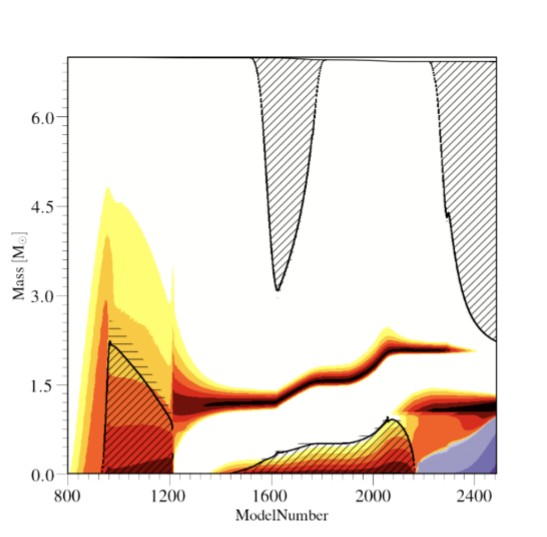
\includegraphics[width=10cm]{plots/Kipp_diagram.png}
    \caption{Kippenhahn diagram massive star. Describing the stages of stellar evolution.}
    \label{fig:KH1}
\end{figure}

\begin{enumerate}
    \item This diagram displays the evolution of the structure of the star from the core to the photosphere. The vertical axis represents the position within the star in terms of enclosed mass and the horizontal axis represents the number of the models which can be translated to the age of the star. In this diagram, we can see how different regions are discerned: The white parts are the radiative regions, the stripped parts represent the convective regions, and the variation of the color represent the intensity of the energy at various regions. Darker color indicate that more energy is produced. 
    \item The advantage of using the model numbers for the x-axis of the Kippenhahn diagram is that we can see the whole evolution in the star with the same resolution, therefore we see more details with wider overview. This happens because the scales in this diagram is adaptive, and the units in the x-axis are not equal in time. However, this implies that we cannot tell how long each process lasts, so that would be the disadvantage. 
    

    \item (a) Central hydrogen burning is taking place from model number 920 to 1200.
    \\
    (b) The enclosed mass in the convective core at the beginning of H-burning is about $2.5 M_{\odot}$
    \\
    (c) The enclosed mass in the convective core at the end of H-burning is about $0.75 M_{\odot}$
    
    \item Between the model 1200-1350 we can observe the thick H-shell burning phase. This happens after the H is completely exhausted inside the core - the core He starts to contract and the temperature increases. At some point the temperature becomes high enough to fuse the H in the shell around the inert core.
    \item (a) The He-burning core can be seen between model 1440 and 2160.
    \\
    (b) The core during the He burning is convective. For the He fusion we have $\epsilon_{CNO} \propto T^{40}$. Hence, there is a huge amount of energy produced, that can be transported only through convection. A shaded area (marking the convection) can be seen in the core's region during the He burning.
    \item The purple region marks the existence of an inert CO degenerate core, the end-product of He fusion in the core. In this degenerate medium, the weak interactions produce lots of neutrinos which take energy out of the star (they don't interact with the normal matter). Thus, the CO core is efficiently cooled down and there is a net loss of energy.
    \item As mentioned before the vertical axis represents the position within the star and the stripped parts represent the convective regions. These can appear either in the core or in the envelope. Convection regions are developed in the envelope during the H-shell burning phase (after the Hertzsprung gap) and during the early AGB phase, when He-shell burning is active. In both situations the convective envelope is formed due to the raise of the opacity, which is a consequence of the mirror principle. During the active shell burning phase, the core contracts and the envelope expands. The expansion of the envelope implies a decrease of the temperature throughout the entire region, giving rise to a higher opacity. Hence, the radiative gradient becomes larger than the adiabatic one and consequently, convection becomes more efficient in transporting energy throughout the star. The convection region is formed, starting from the surface (where T is minimum) and penetrates through deeper layers
\end{enumerate}


\subsection{Kippenhahn diagram for $15M_{\odot}$ star}

\begin{figure}[H]
    \centering
    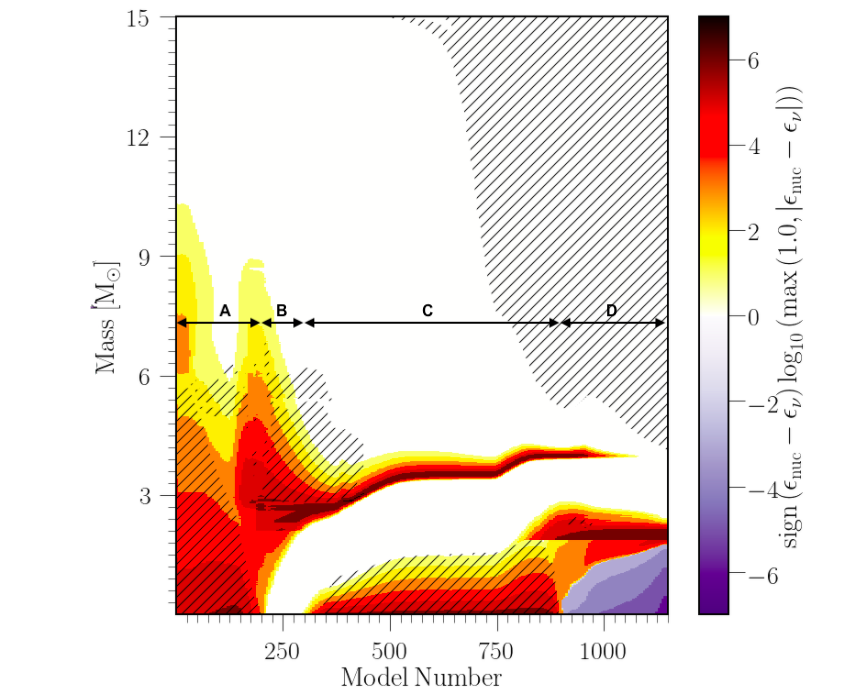
\includegraphics[width=14cm]{plots/Kipp15m.png}
    \caption{Kippenhahn diagram of  massive star with 15$M_{\odot}$}
    \label{fig:KH1}
\end{figure}

\textbf{A}: From model $0$ until model $\sim 200$ we see a convective core, where hydrogen burning takes place, with a radiative envelope. The energy production is most concentrated in deeper layers, where the temperature and the density are higher ($\epsilon_{nuc,CNO} \sim \rho T^{18}_{eff}$). 
\\
\\
\textbf{B}: After model $200$  the hydrogen in the core is depleted and the hydrogen shell burning takes place. It starts with a thick hydrogen shell burning phase and the shell gradually becomes thinner. This goes until model $300$ and during this phase the core is radiative and contracts due to the virial theorem, thus the envelope expands (in $\tau_{KH}$) and the effective temperature reduces. The interesting thing is that in the case of a $15 M_{\odot}$ the thick shell, which burns hydrogen, seems to be convective. This tells us that the shell produces much energy and radiation itself can not efficiently transport it to the surface. Going a step further and compare it with the Fig. \ref{fig:KH1}, where the shell is radiative, we can assume that the $15 M_{\odot}$ has a higher temperature in that shell thus producing more energy (they both burn hydrogen via the CNO-cycle). 
\\
\\
\textbf{C}: From model $300$ until model $900$ the helium burning in the core takes place and simultaneously hydrogen shell burning continues, but inside a thinner shell. The contraction of the core has been ceased. The core now is convective once again, while the burning shell is radiative. The interesting thing here is that the biggest portion of the luminosity is coming from the shell burning and not from the core. Another key feature that we see in the plot is that the envelope starts to become convective during the helium burning phase (starts to climb the Hayashi line). To explain that we need to think the combination of three parameters: The change of composition in the core, the mirror principle (with the hydrogen burning shell acting as a mirror) and the timescales. Until the ignition of helium the envelope was expanding on $\tau_{KH}$, but after that the core starts getting bigger ($\mu \; \nearrow$), thus the envelope should start to contract as a consequence of the thermostatic behavior of the CNO-cycle in the shell. The key here is that the contraction happens on $\tau_{nuc}$, which is $<< \tau_{KH}$, thus the expansion slowly decelerates, but the envelope manages to reach temperatures low enough to rise the opacity and becomes convective. We can also see that the convection is being built from the surface towards the deeper layers, which is normal because further up the layers are colder. Hence, this is a big difference in comparison with the $5 M_{\odot}$ star and tells us that the $15 M_{\odot}$ ignites helium in the core before it starts to climb the Hayashi line.
\\
\\
\textbf{D}: Starting with the model 900, the He-core fusion is quenched and the star enters the (early) AGB phase. The core (He-rich envelope and the CO core) starts to contract in the absence of energy production. Since the He-rich envelope is radiative, the contraction leads to a temperature gradient, from the bottom of the envelope to the outer parts. At some point, the temperature of the bottom part becomes high enough to fuse the He in the shell. Since the H and He fusion are both very sensitive to temperature, these cannot take place simultaneously. The He-shell is thicker than the H-shell and produces more energy. Thus, the envelope above the He-shell expands and the H-shell burning is quenched (because the temperature decreases). From this point on, the star enters a stable phase of He-shell burning, during which the envelope expands and becomes convective (the star enters the Hayashi line for the second time).  Meanwhile, the CO core contracts and becomes degenerate. Due to the electronic degeneracy pressure, the CO core remains in HE while it cools down (blue region marks the loss of energy). The cooling is efficiently done by the escape of neutrinos from the degenerate core.


\bibliographystyle{mnras}
\bibliography{lib}

\end{document}


